\documentclass[12pt]{article}
\usepackage[T1]{fontenc}
\usepackage[utf8]{inputenc}
\usepackage{lmodern}
\usepackage[margin=1in]{geometry}
\usepackage[hidelinks]{hyperref}
\usepackage{graphicx}
\usepackage[english]{babel}
\usepackage{setspace}
\usepackage{enumerate}
\usepackage{titling}
\usepackage{subcaption}
\usepackage[capposition=top]{floatrow}
\usepackage{dcolumn}
\setlength\parindent{0.5in}
%\usepackage{harvard}
\usepackage{multicol}
\usepackage{booktabs}
\usepackage{rotating, graphicx}
%\usepackage[landscape]{geometry}
\usepackage{natbib}
\usepackage[dvipsnames]{xcolor}

\usepackage{tikz}
\usetikzlibrary{positioning}
\usetikzlibrary{shapes.multipart}
\usepackage{subcaption}
\usepackage{emoji}


\title{Police Killings and Voter Turnout \vspace{1in}} 
%\title{Communities Turnout Out in the Wake of Police Killings  \vspace{1in}} 
\author{Kevin T. Morris, Brennan Center for Justice/CUNY Graduate Center\thanks{XXX is the corresponding author: XXX[at]XXX. Kevin T. Morris is a quantitative researcher with the Democracy Program at the Brennan Center for Justice and a graduate student at CUNY Graduate Center. Kelsey Shoub is an assistant professor of political science at the University of South Carolina.} \\ Kelsey Shoub, University of South Carolina}
\date{}

\newcommand{\kscomment}[1]{\textbf{\textcolor{Thistle}{[[ #1 --- KS ]]}}}
\newcommand{\kmcomment}[1]{\textbf{\textcolor{JungleGreen}{[[ #1 --- KM ]]}}}

\usepackage{fancyhdr}
\fancypagestyle{plain}{
  	\fancyhead[L]{{\scA Police Killings and Voter Turnout}} 
	\fancyhead[R]{Paper Draft}
  	\fancyfoot[R]{} 
  	\fancyfoot[L]{} 
}

\begin{document}
%\pagestyle{plain}
\setcounter{page}{0}
\clearpage
\maketitle
\thispagestyle{empty}

\renewcommand{\abstractname}{\vspace{-\baselineskip}}
\begin{abstract}
\noindent Insert abstract.
\end{abstract}

\vspace{1cm}

\noindent \textit{Paper prepared for the 2022 Southern Political Science Association Annual Conference in San Antonio, Texas. Please do not cite or circulate without the permission of the authors.}

\pagestyle{plain}

\newpage
\doublespacing

\kscomment{I essentially went from the Intro (didn't touch the reg stuff here yet) through the initial test. Then I cleaned up the *potential* outline for that last theory section. I think the big question continues to be what to do about registration. To me the options are: (1) lump it in with turnout and sweep some of the weirdness under the rug and just add "registration and turnout" in rather than just "turnout" to the theory + expectations; (2) we include it as a test looking at another form of participation; or (3) say something like ``if communities tap into this framework and organize, we'd expect longer term effects as it's no longer a gut reaction'', which in turn would lead us to look for a test of a related something that can be long run -- i.e., registration.}

\kmcomment{Okay--I made some small changes to the main theory section (mostly tried to do something on the violence question). I also took a first pass at laying out the second theory section using your outline and seeing what flowed (for me). Ended up spending a lot of time with Hannah's work, and also bringing in the political threat literature pretty explicitly. Since we hit a lot of this earlier, this section is pretty short---about 2 pages. I also explicitly lay out hypotheses for the tests there. It feels like the registration test works nicely in this setup, but curious about your thoughts.s I also tried to clean up the RDiT section where you were confused. And then laid out a first potential paragraph for the discussion, but since you have a pretty detailed outline there / seems like there's particular literatures you want to tie to, it might be better for you to take the first pass for the rest (though I'm happy to help).}

\kmcomment{My main remaining question at this point is with respect to the second theory section / second set of tests. As currently written we do 1) nhood demos theory, 2) registration theory, 3) support for abolition theory, 4)nhood tests, 5) reg tests, 6) minneapolis tests. Does this feel like too much back and forth? I *think* I like this best, since the theory is all super related. But the back-and-forthness of these sections might be a little too confusing. Something to think on}

\section*{Introduction} % We'll delete the introduction header later. It's just convenient to leave in now for navigation purposes.

%\begin{itemize}
    %\item How do police killings, where an officer kills a member of the public, affect political participation? One documented response has been protesting — at least by Black communities when the police shoot and kill a Black person (CITES). However, less is known about how such tragic events impact more traditional forms of participation that work within the system. In other words, we know less about how police violence relates to voter turnout and registration. 
%\end{itemize}

\kscomment{We need to work registration in somewhere.}
\kmcomment{I took a stab, but the way I've written it in the intro is as an extension of the turnout treatment, not an investigation of why / how police killings mobilize / part of the narrative piece. I guess I'm still not super clear on how the registration test gets us something different than the turnout piece. How exactly are you thinking that the timing of the registration effect gets at this puzzle? I know you've tried to explain this to me 100 times and I'm being obtuse but not on purpose, I swear} \kscomment{Haha, I don't think I've done a good job explaining it, which would make sense as to why it doesn't make sense. Partly that's because we've been going back and forth as to what the results are and how they fit in. }

In 2020, the police shot and killed over 1000 people in the United States -- which is not an anomaly in the US. Each year between 2015 and 2019, just under 1000 recorded deaths occurred during police interactions \citep{sullivan2019four}. 
% https://www.washingtonpost.com/investigations/four-years-in-a-row-police-nationwide-fatally-shoot-nearly-1000-people/2019/02/07/0cb3b098-020f-11e9-9122-82e98f91ee6f_story.html
Some of these shootings ignited protests -- both locally, such as the death of David Jones in Philadelphia \citep{davidjones}, and nationally, such as the murder of George Floyd in May of 2020 \citep{georgefloyd}--, and they spurred on political activism and movements pushing for change, such as Black Lives Matter and \#DefundThePolice. Initial studies find greater police reform occurring in areas where protests occurred \citep{olzak2021does} and that they -- at least temporarily -- shifted public opinion \citep{Reny2021,wasow2020agenda}. 
% https://www.usatoday.com/in-depth/graphics/2020/06/03/map-protests-wake-george-floyds-death/5310149002/
% https://www.bloomberg.com/news/articles/2020-06-09/a-history-of-protests-against-police-brutality
However, it is unclear whether such killings \textit{typically} spur on political action and activism, as we know not all incidents garner media attention nor spur protests. Further, few studies have questioned whether police killings are linked to other forms of political participation commonly studied, such as voting, which is the focus of this paper.  

Prior research provides conflicting expectations on whether the public -- even locally -- may be mobilized to register and vote in the wake of a police killing. 
Research on contact with the police and carceral state tells us that personal contact demobilizes \citep{burch2011turnout,lerman2014arresting,weaver2010political,white2019misdemeanor}, while proximal contact can \textit{sometimes} mobilize people with respect to extra-voting activities and has no relationship with voter turnout \citep{walker2014extending,walker2020mobilized,white2019family}.  
%Research on proximal and personal contact with the police and carceral state tell us that while contact can \textit{sometimes} mobilize people with respect to extra-voting activities, such as protesting, personal contact typically demobilizes with respect to voting\citep{burch2011turnout,lerman2014arresting,weaver2010political,white2019misdemeanor}, while proximal contact appears to have no relationship with turnout \citep{walker2014extending,walker2020mobilized,white2019family}. 
%Conversely, research on place-based mobilization, tells us that voter turnout may increase in the wake of local, community tragedy and hardship, where a narrative exists that connects an event to a cause to political action, such as local government closing schools \citep{nuamah2021close} -- or potentially in the case of local police shootings.
Conversely, research on place-based mobilization tells us that voter turnout may increase in the wake of localized (negative) policy change, such as the local government closing public schools, where a narrative connects an event to a cause to action \citep{nuamah2021close}. Extending this framework to local tragedies and hardships whose source can be tied to government policy or action -- such as local police killings --, prompts a similar expectation: those with \textit{community contact} with the police may be expected to turn out at higher rates.  %\kscomment{Could add: Note that with both personal and proximal contact on the one hand and community contact on the other political learning may occur. However, the former results in learning via direct interactions or pragmatic research, while the latter results in learning via the media, community conversations, and local activists.}
%As such, we first ask: How do these events affect political participation, and how do we reconcile these theories? 

To test these competing expectations, %To that end, 
we, first, offer a novel empirical study of the effect of police involved killings on voter turnout levels in 2016 and 2020. We use a series of snapshots of the national voter file to estimate turnout for each Census block group. We leverage the random timing of a police killing shortly before or after election day and a regression discontinuity in time (RDiT) approach incorporating state-of-the-art econometric recommendations \citep{Calonico2014, Stommes2021} to measure whether turnout was higher in neighborhoods with a police killing immediately preceding election day. We find that local communities within a half-mile of a police killing turn out to vote at higher rates. Our RDiT approach allows us to estimate the local average treatment effect, which can answer only whether a police killing influences participation if it occurs \textit{immediately before} the election. To explore the temporal nature of the effect of a police killing on political participation, we also estimate a two-way fixed effects model \citep{Callaway2021} testing the effect of police killings on block-group level weekly registration counts in 2020, finding that block groups near police killings do see increased registrations---but that this treatment effect is concentrated not in the weeks following the police killing, but in the weeks preceding the registration deadline.
%This suggests that indirect community contact with the police results in a different response than direct contact. %-- be it personal or proximal.
%Using a differences-in-differences approach \citep{Callaway2021}, we also find evidence that weekly registration counts increase in neighborhoods close to a police killing. These findings suggest that indirect community contact with the police results in a different response than direct contact -- be it personal or proximal.

These findings on the political implications of police killings prompts the question of why. 
One explanation is that the narratives surrounding police killings allow \textit{local} communities to understand and respond to the tragedy that has occurred \citep{nuamah2021close,stone1989,walker2019targeted,walker2020mobilized}: the killing was caused by specific policing practices, which can be addressed through a change in policies or through a change in who is elected to office (i.e., by voting). %This points to a government cause that can be addressed by community involvement in government (i.e., by voting). 
Further, these narratives may be particularly strong if they resonate more with the community or specific killing. In the United States, this narrative may be particularly salient among Black communities or when a Black individual is killed \kscomment{Cites}. 
%While some have similarly proposed that narrative can structure responses of those with personal and proximal contact \cite[e.g., ][]{walker2020mobilized}, community contact differs in three significant ways: (1) it does not directly place practical burdens on those effected, which \cite{white2019family} hypothesizes is what demobilizes those with proximal contact in the short run; (2) unlike personal contact, it carries fewer alienating stigmas \citep{lerman2014arresting,lee2014consequences}; and (3) personal and proximal contact produce learning via direct interactions or pragmatic research, while community contact produces learning via indirect sources, such as the media, community conversations, and local activists. 
This further implies two things: (1) mobilization effects will be more pronounced among groups where the narrative resonates (i.e., predominately non-white communities) and in instances where it more closely matches what occurred (i.e., the victim is not white); and (2) proximity to shootings will increase support for abolishing or defunding the police. 

To test each, we turn again to our neighborhood-level turnout estimates and demonstrate that the turnout effects we observe are concentrated in Black neighborhoods and when the victim is Black. Of course, knowing \textit{that} Black neighborhoods turned out at higher rates following an extrajudicial killing provides little evidence on \textit{how} they voted. To that end, we turn to precinct-level results from a Minneapolis ballot initiative in 2021 that proposed abolishing the police. We show that voting precincts that were closer to a police killing were more supportive of abolishing the police, even after accounting for the prevalence of low-level police stops. While this relationship is not causal, it is consistent with a causal mechanism that leads voters exposed to police violence to (a) be less supportive of the police, and (b) turn to the ballot box to voice that displeasure.

%Investigating the effects of police violence is important for XXX reasons. \kscomment{Expand.}

Across the two pieces of our study, we find that police killings can electorally mobilize local communities that this is more pronounced among communities where narratives are more likely to resonate. %where narratives of the ill effects of policing practices are more likely to resonate. 
In doing so, our study makes three key contributions. First, we advance our understanding of local political mobilization by distinguishing between three types of contact -- personal, proximal, and community -- in the context of the police contact. We show that, in contrast to personal and proximal contact, community contact can mobilize voting. In doing so, we extend the theory of place-based mobilization to span not just sudden, geographically bound policy changes but also events that can be tied to government policy or action. 
Second, building on prior work that focused on specific localities that may be unique in their histories or contexts, we construct a national test showing mobilizing effects across the United States. Finally, our use of geocoded national voter files coupled with advanced statistical causal estimation methods joins a growing body of work \cite[e.g.][]{TamCho2013, Hersh2016, Brown2021} that uses hyper-local data to understand political processes that are geographically-bounded. % and thus unobservable using more traditional methods and approaches. %Beyond contributions to the academic literature, \kscomment{Broader, perhaps normative, statement here}.
%\begin{itemize}
%    \item \kscomment{Why is this important? What does it contribute?}
%    \begin{itemize}
        %\item Bring cutting edge methods to bare.
        %\item Test a portion of the mechanism that may be at play: narratives + re-purposing activist tools.
        %\item As such, contributes to our understanding of multiple literatures (i.e., local political mobilization, policing + political mobilization, and XXX)
        %\item Also ... \kscomment{Broader, perhaps normative, statement here}
%    \end{itemize}
%\end{itemize}

\section*{Community Contact and Turnout}%Motivating (or Depressing) Community Participation}
%\kscomment{Initial thoughts from e-mail chain.} \kscomment{Lit/Theory: Either competing hypotheses or fully push for one. Do we want to put all of the theory in one place?}

%\kmcomment{I think I prefer community to tertiary contact, but not necessarily strongly. At a more theoretical level, I also wonder if distinguishing proximal from community via the learning mechanism makes sense. What I mean by this is, with proximal contact, you see the state \textit{acting on} someone you know / love. The state's action is mediated through a known individual. With community contact / a killing, on the other hand, you might not have known the person or they might be more abstract. You might see the state acting on an Joe Anybody, which surely would politicize differently than via a loved one's experience. Not sure if this matters here or is interesting though.} \kscomment{I think that's right, and that's what I'm trying to slowly build out in the theory section! An extension or alternative here might also be: rather than direct learning via interacting with the system or helping to deal with the system *in that moment* you learn about the system via the media, community conversations, and activists.}

%\kscomment{KM: We could greatly expand this section. The question is whether we need to and if yes whether we need to expand each point or just certain points. Also, I dropped the school shootings bit from here (now in the notes and spare writings folder), and I also broke out proximal + personal contact into two different hypotheses.}
 
%\kmcomment{I think this section is pretty good as-is, but have two thoughts / comments: 1) I really think we need to incorporate the Laniyonu paper somewhere. I can take a stab at that. Since that's community turnout / response to turnout, I think it's relevant here. 2. I wonder whether we need to deal with violence *specifically* here or not. Is contact with a *violent* carceral state different than contact with other manifestations? I don't think we can really answer that, but probably something we should note} \kscomment{Change and edit whatever! I agree on the violence bit...I was trying to figure out how to incorporate that here. If you can, please do. Regardless, I think this is an A+ thing for us to bring into the discussion section and lets us tie into the survey experimental lit that's been looking at some of this.} \kscomment{Also, if there are other or larger changes you think we should make, I'm 100\% on board. Needs tightened up.}

Depending on the theoretical lens one extends to study how community contact with officer involved deaths relates to political participation, expectations vary -- as do expectations based on the type of participation studied, with many finding distinct patterns when looking at voting compared with other forms of participation, such as protest and contacting elected officials \citep[e.g., ][]{walker2020mobilized}. 
%Depending on the theoretical lens one uses to study police killings and political participation expectations concerning political participation and mobilization vary, as do expectations based on the type of participation studied, with many finding distinct patterns when looking at voting compared with other avenues of participation, such as protest and contacting elected officials \cite[e.g., ][]{walker2020mobilized}. 
Unlike many prior studies, which have examined protest \citep{williamson2018black}, public opinion \citep{Reny2021,wasow2020agenda}, educational outcomes \citep{ang2021effects}, and government contact \citep{cohen2019officer} in the wake of police shootings, we focus on voter turnout, as it is one of the most common forms of political participation and closely tied to who holds elected office. 
%Voting differs from other forms of participation as \kscomment{Voting compared with other forms of participation aka why we expect it to be different}. 
So, how might police killings relate to voter turnout? Does the ballot box appear an appropriate means of addressing political violence in citizens' communities? We construct a trio of competing expectations by drawing from and extending three areas of research. %: (1) treating community contact with the police through police killings as similar to personal or proximal contact with the the police or carceral state \citep[e.g., ][]{white2019family,walker2020mobilized,lerman2014arresting}, (2) instances of (group) violence in the United States that may be considered black swan events \citep{hassell2020mobilize,garcia2021violence}, and (3) an extension of a theory of place-based mobilization \citep[i.e., ][]{nuamah2021close}. \kscomment{One question for us to think about is whether we want to or should connect to any comparative work on this topic -- if it exists. }

Prior work on contact with the police and carceral state has primarily focused on personal contact, which is first-hand or direct contact an individual has with the police or carceral state (e.g., they are arrested), and proximal contact, which is close but second-hand contact an individual has with the police or carceral state (e.g., a family member, friend, or loved one is been arrested). 
%These studies find a demobilizing effect of personal and proximal contact on voting -- at least in the short term \citep[e.g., ][]{weaver2010political,lerman2014arresting,white2019misdemeanor,walker2020mobilized,walker2014extending,white2019family}. 
Scholars studying personal contact tend to focus on two explanations for how such contact structures participation in electoral politcs: (1) resources are stripped from an individual, such as time and funds, such that they cannot participate even if desired; and (2) it alienates and stigmatizes individuals by communicating that they do not belong, which in turn means that they should not participate in government or the system. As such, these studies hypothesize that the likelihood of voting immediately following contact decreases, as voting is a form of participation directly tied to our understanding of ``who counts" and political belonging. Support for this proposition has been seen regardless of the test conducted be it with survey data \citep[e.g., ][]{lerman2014arresting,weaver2010political}, which additionally show greater substantive relationships for harsher forms of contact, or causal estimates generated using observational data \citep{white2019misdemeanor}. Additionally, similar patterns have been shown for those with personal contact with other government bureaucracies that stigmatize or transmit messages that one does not belong \citep[e.g., ][]{soss1999lessons,michener2018fragmented}. 

%A key distinction between personal and proximal contact is that costs incurred by personal contact, in the form of time and material resources, may not be incurred with proximal contact. 
However, our focus here is on \textit{community contact}, which is diffuse contact an individual has with the police via community incidents, word of mouth, the media, \kscomment{refine the def} rather than personal contact with the police. In other words, this sort of contact comes not from direct, personal experience, nor the experience of a loved one---it is, rather, mediated through an individual's relationship with their community. \kmcomment{Adding this sentence only to really hit home how this differs from proximal. Can cut if we think it's redundant} While she does not call it community contact, \cite{burch2013trading} questions whether greater levels of surveillance in the form of higher rates of contact with the carceral state (i.e,. higher incarceration and parole rates) relate to differential levels of \textit{community} political participation. She finds that communities with high incarceration rates or where a significant portion of the community is formally incarcerated perceive and internalize messages that they do not belong and that communities under greater supervision turn out to vote at lower levels. \cite{Morris2020} similarly finds evidence that the recent incarceration of community members 
%with recent histories electoral participation 
reduces neighborhood-level turnout. Both Morris' (2020) and Burch's (2013) work further focus is local, which we adopt here as well. Together with the work done on personal contact, this implies that: \textit{In the surrounding community, voter turnout will be lower following a police killing} (\textit{H1a}). 

Conversely, recent political science studies of proximal contact have found either no relationship or a limited demobilizing effect between proximal contact and voting. Scholars point to two key distinctions between personal and proximal contact to explain these results. First, the costs incurred by personal contact, in the form of time and material resources, may not be incurred with proximal contact and to the extent that they are it is to a lesser degree. Second, the alienating messages transmitted in personal contact are more distant or not applicable to those with proximal contact. Again, recent studies turning to both survey data \citep{walker2014extending,walker2017love,walker2020mobilized}, and to causal estimates generated using observational data \citep{white2019family} find no relationship between turnout and proximal contact in the long run. While none of these studies show longterm associations between proximal contact and voting, \cite{white2019family} does find short term effects, which she attributes to an immediate resource drain and associated disruptions. Further, multiple studies have shown increased likelihoods of politically participating in ways other than voting, such as protesting or contacting elected officials, among those with proximal contact \citep[e.g., ][]{walker2019targeted,walker2020mobilized}, and that closer proximal ties are associated with larger substantive relationships \citep{walker2014extending}. 
%\kscomment{Could add 1-2 sentences here that brings back the school shootings bit.}
As community contact may be a broader form of proximal contact, this implies that: \textit{In the wake of an individual being killed by the police, turnout will remain unchanged} (\textit{H1b}).

%We should note however that those with proximal contact may reject this alienation narrative. As \cite{walker2020mobilized} argues this is likely to happen if they can connect their loved ones contact to an injustice narrative: \kscomment{XXX}. Indeed, she finds that for forms of participation other than voting those with proximal contact with whom an injustice narrative resonates are more likely to mobilize.

%However, as this literature primarily focuses on relatively close contact with the police or carceral state and not community contact, there are questions whether this may generalize to those experiencing community contact only. To that end, we can draw a parallel to another form of violence that often affects \textit{communities} in addition to those who personally and proximally experience them: school shootings, which are relatively rare but are viewed as a community tragedy. Research questioning the (de)mobilizing affects of school shootings suggests that communities turnout to vote at the same rates as before a shooting took place, as research on political behavior indicates that voting decisions are entrenched and difficult to change \citep{garcia2021violence,hassell2020mobilize}. We should note that each of these studies situates school shootings differently than we do here and each pulls form distinct theoretical traditions: \cite{hassell2020mobilize} do so with reference to disasters and retrospective voting and additionally find that incumbents receive lower vote shares following such events; and \cite{garcia2021violence} do so with reference to (group) political violence and further find that Democrats capture a greater share of the vote following rampage style shootings. Both research on proximal contact and research on school shootings point to the same expectation: \textit{In communities where a police killing recently occurred, registration and turnout will remain unchanged} (\textit{H1b}). 

%There are two, key, theoretical differences between school shootings and police killings. First, how they may be  \kscomment{Two key differences. Group violence + terrorism vs isolated acts of state violence.}
%neither school shooting paper talks about shootings in the context of contact with the event. Rather one does so with reference to black swan events/disasters. The other talks about them with reference to (political) violence concerning group events.

%A key difference between school shootings and police killings are the narratives that surround each -- and specifically how each assigns blame and whether and how the public should react. \kscomment{What are narratives; how do the structure behavior; why do they matter here} 

While prior work on personal and proximal contact and on the effects of surveillance via incarceration on communities has provided key insights in this space, our focus may be sufficiently distinct that different theoretical mechanisms may be more appropriate. Community contact by definition is distinct from both personal and proximal contact; it is both more distant and diffuse. However, that may not be its only distinctive feature. Officer involved shootings leading to a civilian death may also be distinct compared with other forms of police contact. It is an extremely harsh form of contact and is significantly rarer. Moreover, some individuals in over-policed and incarcerated neighborhoods still believe in the central fairness of the criminal legal system, locating patterns of incarceration in community-member's behavior and not structural conditions \kmcomment{cite}. Extrajudicial killings by the state, however, are more likely to violate an innate sense of justice given the central place a trial by a jury of one's peers has in American culture. Further, there is far lower support for the death penalty than for other forms of punishment \kmcomment{cite}, perhaps leading to a unique response to extreme police violence. Finally, anecdotally, shootings appear to be much more likely to make the news, have spurred on both local and national protests, and legislators name bills aimed at reforms after victims. As such, looking outside of the direct literature on political participation and contact with the criminal justice system and turning instead to a related literature on place-based mobilization and responses to policy threat may prove fruitful. 

In their theory of place-based mobilization, \cite{nuamah2021close} describe how citizens respond to geographically concentrated policy change, where mobilization and engagement are based on community context. Geographically concentrated policy effects have three key characteristics: (1) they occur in some geographical areas of a city or state but not others or at least more so than in other areas; (2) members of the community who are not directly, personally affected can still discern and feel the effects of the policy; and (3) members of the community understand the policy change as particularly targeted at them, which is communicated via narratives. In the face of negative geographically concentrated \textit{negative} policy effects -- or in the face of geographically concentrated policy threat --, community members will then mobilize to oppose them. For example, in 2012 Chicago initiated the closure of 49 public schools throughout the city and disproportionately targeted communities of color, which narratives surrounding the closures clearly stated. In the wake of these closures, \cite{nuamah2021close} document increased mobilization, both with respect to turnout and other forms of participation, and an uptick in support for reform of the structure of the city's school board. More generally, as \cite{garciarios2021implications} discuss, communities of color, particularly Black Americans, have both a group consciousness and understand that many government polices are targeted at their community, which means Black Americans are more likely to mobilize in the face of negative policy changes that effect their local community.   

This corresponds with what some have found with respect to the mobilizing effects of threatening immigration policy on Latino communities \citep{pantoja2003fear,barreto2009mobilization}\kmcomment{YES! Was just thinking of political threat lit yesterday for this. Love} and what \cite{Laniyonu2019} finds in his exploration of the effect of Stop, Question, and Frisk stops in New York City. After finding evidence that these low-level police stops were associated with higher turnout at the neighborhood level in local and presidential---but not midterm---elections, he concludes that, ``in electoral contexts \textit{which present communities with an opportunity to address the threat or harm constituted by policing,} policed communities may mobilize to counter-act that harm'' \citep[][551, emphasis added]{Laniyonu2019}. In other words, policy threat targeted at specific groups can increase voter turnout. 
%While this mobilization may begin with non-electoral actions, they are theorized to develop into or expand to include such activity. 

%\kscomment{I need to fix this chunk.} 
%A key facet of this theory is the role that narratives play, as narratives \kscomment{role of narratives}. In the case of school closings, they highlight how \kscomment{racism + systemic things}. 

While both the Nuamah and Ogorzalek's (2021) place-based mobilization theory and these policy-threat based explanations center on responses to specific (proposed) policies, the underlying logic may also apply to events that are understood to be caused by government or government policy. Events or incidents occur within a geographic area, and are likely to impact those in the immediate area to a greater extent than those farther away. Additionally, those in the immediate area may be more likely to know something happened via local media, (online or in person) community groups, or local organizations, which means even though they are not directly, personally affected they can still discern the effects of the incident. Finally, narratives or the causal stories we tell about these events can connect government action or policy to the specific outcome by way of targeting a specific group. 
In other words, these theories may not only apply to specific policies but also to incidents or events stemming from broader policy or action. 

In the case of officer involved shootings and killings, one of the dominant narratives is that they are the result of systemic forces: predominately Black neighborhoods are aggressively and overly policed not necessarily to increase public safety but rather to maintain control, which results in the unnecessary and unjust deaths of Black people at the hands of the police. In other words, there is a narrative of racial injustice perpetuated and perpetrated by the police, an arm of government. Examples of the prevalence of these narratives can be seen in the coverage of the death of Breonna Taylor and the murder of George Floyd. In the wake of each death, the public mobilized and called for specific policy changes ranging from specific changes, such as barring no-knock warrants and choke holds, to abolishing the police. \kscomment{Do we need cites for these?}\kmcomment{I don't really think so. Seems like general knowledge} These narratives recognize government as the cause, so to address it one must change the government. Prior movements and pushes for policy change provide blueprints for how communities can push for such change: by organizing and then mobilizing, includes going to the polls. %, just as \kscomment{connect to historical movements}. 
Indeed, this corresponds with work done by  \cite{walker2019targeted,walker2020mobilized} on proximal contact\kmcomment{Doesn't the book also find this for personal contact? Could be mis-remembering}, which shows that greater internalization of the injustice narrative is linked to greater non-electoral, political participation among those with proximal contact. 
In this vein, \cite{jefferson2021seeing} and \cite{burch2021notall} document that Black Americans seem to process information about officer involved deaths differently than their white counter parts -- at least in some instances -- using survey data. 
%This corresponds with what \cite{Laniyonu2019} finds in his exploration of the effect of Stop, Question, and Frisk stops in New York City. After finding evidence that these low-level police stops were associated with higher turnout at the neighborhood level in local and presidential---but not midterm---elections, he concludes that, ``in electoral contexts \textit{which present communities with an opportunity to address the threat or harm constituted by policing,} policed communities may mobilize to counter-act that harm'' \citep[][551, emphasis added]{Laniyonu2019}.
%Here specifically, this suggests that if the police killings can be tied to a broader narrative that indicates specific action items then one would expect communities to be mobilized in the wake of tragedy, as they are in the wake of geographically constrained policy change and in response to targeted policy threat. 
Together, this implies that: \textit{In communities where a police killing recently occurred, voter turnout will increase} (\textit{H1c}). 

In sum, we draw on multiple literatures to construct competing expectations as to whether and how officer involved killings relate to voter turnout. Prior studies of personal contact with the police indicate that a killing should decrease turnout (\textit{H1a}), while prior studies of proximal contact with the police indicate there should be no relationship (\textit{H1b}). Conversely, an extension of a theory of place-based mobilization to events whose blame can be placed on government lead us to expect an increase in turnout in the wake of an officer involved killing (\textit{H1c}). Following previous studies, our focus is on whether turnout increases, decreases, or stays in the same in the geographically proximate area. As such, in the tests we turn to in the following sections, we test the turnout of census block groups near a police killing immediate the 2016 and 2020 elections relative to those near killings immediately afterwards.\kmcomment{is this the sort of thing you had in mind for here?}

%\kmcomment{High level comment on the value of registration *and* turnout tests. Turnout is perhaps more substantively more important, BUT the registration test allows us to test like the temporal nature of the treatment. Is this an immediate / short lived thing, or is it more durable? Moreover, although the RDD can only estimate the LATE, I *think* that the registration test gives us a leg to at least gesture to the possibility that the LATE is more generalizeable, because we see registration effects even many many weeks after the treatment} \kscomment{Awesome. I thin this is something we put in the introduction and then more solidly incorporate/flesh out in the second round of investigations aka in the Group and Place Based section.}

%\kscomment{in sum paragraph -- 1-3 sentences -- that hits home the competing hypotheses? just do that in the analysis?}

\section*{Data on Officer Involved Deaths}
To identify where officer involved deaths occured, 
%police killings occurred, 
we rely on data about extrajudicial killings from two sources: the \texit{Washington Post's} Fatal Force Database\footnote{\url{https://www.washingtonpost.com/graphics/investigations/police-shootings-database/}} and the Mapping Police Violence project\footnote{\url{https://mappingpoliceviolence.org/}}. The Fatal Force data extends back to the beginning of 2015, while the Mapping Police Violence data begins in January of 2013. Since January 1, 2016, these two datasets record 6,481 unique police killings. We turn to these commonly-used open sources of data rather than relying on official government sources because of growing evidence that official sources systematically under-report police violence: According to a paper recently published in \textit{The Lancet}, fewer than half of police killings between 1980 and 2019 were reported in the USA National Vital Statistics System \citep{GBD2019PoliceViolenceSubnationalCollaborators2021}. Instead, the Fatal Force collected by the \textit{Washington Post} data is compiled by ``culling local news reports, law enforcement websites, social media, and by monitoring independent databases'' \citep{Tate2016}. The Mapping Police Violence data, meanwhile, comes from official use of force data collection programs in some states and the crowdsourced Fatal Encounters database. Although the Fatal Force data includes only information about individuals killed by a police \textit{shooting}, Mapping Police Violence includes all known killings, regardless of how the individual died.

We include all police killings that appear in at least one of the two datasets, with most police killings are observed in both datasets (87\%). Of the 6,481 deaths in either data set, about 81\% of these records are already geocoded. For the remaining 19\% of records lacking geocoding, 
%by either the \textit{Washington Post} or Mapping Police Violence, 
we geocoded killings by the data providers using the Texas A&M GeoServices\footnote{\url{https://geoservices.tamu.edu/}} tool. We retain only those records coded with at least 95\% certainty. Between the original providers and the Texas A&M tool, we have the coordinates for 91\% of all killings that occurred between 2016 and 2021 recorded in these data sets. To be sure, these datasources do not include all officer involved deaths: as Mapping Police Violence says, ``there are undoubtedly police killings that are not included in our database (namely, those that go unreported by the media)'' \citep{MPV}. Despite these caveats, these data are the best available for understanding the timing and location of American police killings.

%For our primary voter turnouts models below, 
For our turnout tests, we look at killings that occurred in the two months before or after the presidential elections in 2016 and 2020. As the map in Figure \ref{fig:map-chunk} makes clear, these police killings occur around the country. While they are concentrated in urban areas, nearly every state in the country saw a police officer kill someone in this 4 month period.\footnote{There were just 3 states (Arkansas, North Dakota, and Rhode Island) plus Washington, D.C., that saw no police killings in the 2 months before or after the 2020 election.\kmcomment{JFC this is bananas}}

\begin{figure}[!t]
\centering 
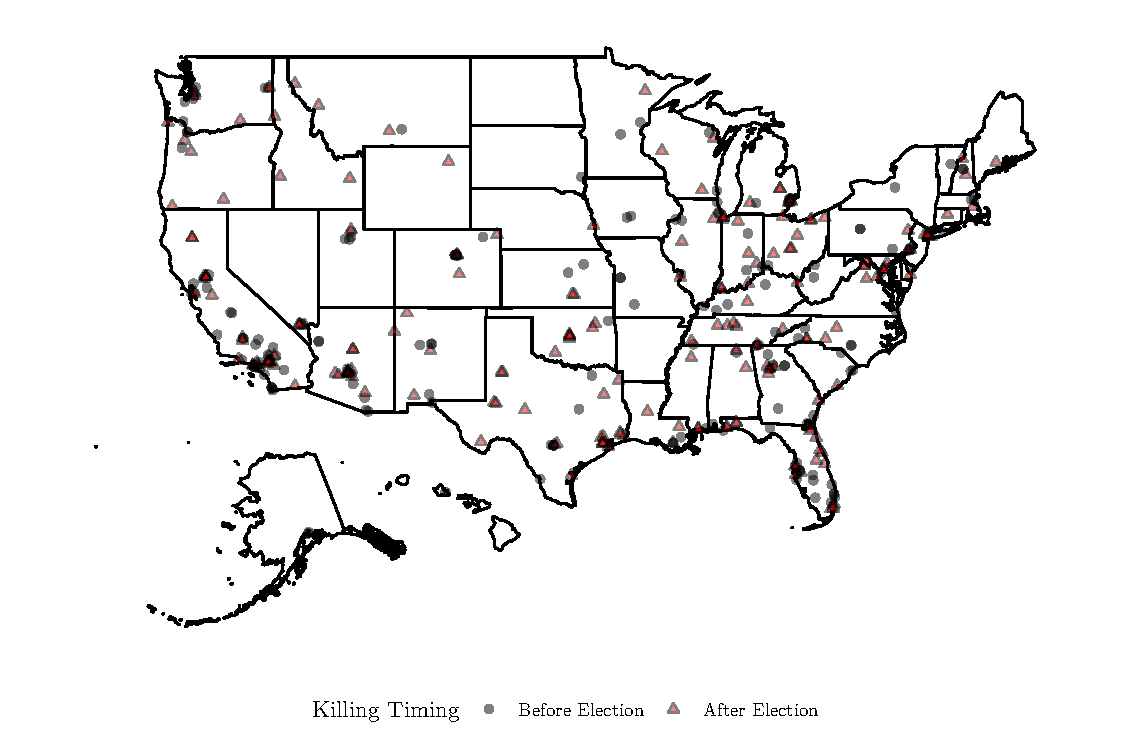
\includegraphics[width=\linewidth]{Figures/map-1} 
\caption{Police Killing within 2 Months of 2020 Election}
\label{fig:map-chunk}
\end{figure}

Neighborhood proximity to a police killing is determined using spatial datasets known as ``shapefiles.'' Shapefiles are made available by the U.S. Census Bureau for each block group in the country, and precinct shapefiles for the city of Minneapolis are made available by that city. We measure the distance between each neighborhood's geographical center (``centroid'') and the nearest police killing.

\section*{Testing the Effects on Voter Registration \& Turnout}

\kscomment{I stored the original version of this in "Notes and spare writings."}

We begin by exploring whether extrajudicial police killings structure voter turnout in the surrounding area. To do so, we leverage two datasets: Snapshots of the registered voter file, and citizen voting age population estimates from the U.S. Census Bureau. In every state in the country (with the exception of North Dakota), voters are required to register on or before election day. 

L2 Political collects and distributes these registered voter files, which are widely used in political science research. Importantly, these records are geocoded, include their registration date, and indicate whether voters participated in a given contest. We specifically use snapshots of each state's registered voter file from L2 shortly following each of the 2014--2020 federal elections. By aggregating these individual-level turnout records, we can precisely estimate the number of ballots cast in each block group for the 2014, 2016, 2018, and 2020 elections. Turnout estimates from 2014 and 2018 are used as controls in our primary models.

Measuring turnout as a share of \textit{registered voters}, however has theoretical drawbacks, as voter files are not always reflective of who is currently residing in the area and eligible to vote, an especially acute problem when the treatment under study might impact registrations \citep[see][]{Nyhan2017}\kmcomment{adding a bit back to this sentence to explicitly cite to the AJPS paper---we can trim it back though if you want}. To circumvent this problem, we calculate turnout by dividing the number of ballots cast in each block group by the citizen voting age population (CVAP) of that block group. Turnout in each year uses the 5-year CVAP estimates ending with the year of that election. \kmcomment{The Census Bureau has said they'll release 2020 estimates next year. Fingers crossed.} \kscomment{What are we using now instead?}\kmcomment{5 years ending 2019. The Census Bureau was originally going to just use the census from last year with Trump's citizenship q to estimate CVAP, but that (blessedly) got scrapped. Of course, there's no reason to think that the CVAP estimates are going to be more biased on one side or other of the cut-point, so we \textit{could} just use the 2019 estimates when we submit, knowing that we'll likely be able to change for an R\&R, and be explicit about how this problem doesn't really matter given our empirical setup} Although these 5-year estimates understate the CVAP where the population is growing quickly, this denominator is far less related to our research question that the number of registered voters in a block group. There is no reason to suspect it introduces meaningful, systematic bias into our analysis.

%After calculating the turnout for each block group in the country in 2016 and 2020, we run a regression discontinuity in time. 
Using the calculated turnout for each block group in the country in 2016 and 2020, we leverage a regression discontinuity in time (RDiT) to test whether proximity to police killing relates to turnout. 
%The regression discontinuity framework is among the most commonly used non-experimental methods used to assert causality in the social sciences. 
%in the social sciences due to the relatively weak assumptions needed to assert causality. 
%Regression discontinuity one side of that cut-point receive a treatment, and those on the other side do not.
An RDiT requires that there be an observable ``cut-point'' date, where observations on either side of a given date can be compared, with only observations on one side of the cut-point receiving the treatment. The cut-point must also be unrelated to the treatment.
%In our analysis, election day serves as the cut-point. 
Here election day serves as the cut-point, and we assume that officer involved shootings occur as if at random with respect to election day. 
More specifically, block groups that were near a police killing \textit{before} election day are viewed as in the treatment group, while those near a police killing \textit{after} election day are considered controls. 
%Of course, block groups near a police killing follow the election are still ``treated'' by a police killing. 
Because a police killing that occurs after election day cannot influence turnout, any discontinuity in turnout between pre- and post-election treated block groups can be attributed to the police killing. 

To make credible causal claims using the RD framework, observations on either side of the cut-point must be virtually identical in all ways except for their placement relative to the cut-point. As we show in Table \ref{tab:balance-tab-full} below, there is some reason to believe that this assumption may not hold in our study. As the table makes clear, in both 2016 and 2020, block groups where a police killing occurred before the election are whiter; less Black; and had higher turnout in the previous midterm election. The table displays the characteristics of all block groups whose centroid was within 0.5 miles of a police killing in the 60 days before or after the election.

To remove these differences between observations on either side of the cut-point we employ what is called entropy balancing \citep{Hainmueller2012}, which has been used to improve the validity of regression discontinuity designs in past political science research \citep{Hainmueller2015}. Entropy balancing assigns control observations unique weights, such that the control group mirrors the treatment group along a set of identified covariates. Here, block groups where a police killing occurred after the election are weighted such that they mirror block groups where a killing occurred before election day. Table \ref{tab:balance-tab-full} shows that this weighting process was successful at removing systematic differences between observations on either side of the cut-point. In addition to entropy balancing weights, we use OLS covariate adjustments in the local linear equations with the same variables. In the Supplementary Information, we show that our results continue to hold even if we use only entropy balancing; only OLS covariate adjustment; or no adjustments at all. Similarly, our results hold when our dependent variable is not turnout in 2016 and 2020, but \textit{change} in turnout between 2014 and 2016, and 2018 and 2020.

Our RDiT models are estimated using the \texttt{rdrobust} \citep{Calonico2015} package, which implements the recommendations of \cite{Calonico2014}: namely, the estimation nonparametric bandwidths; bias-corrected point estimates; and robust standard errors. We thus sidestep the major problems recently associated with RDD designs \citep{Stommes2021}. We use a local polynomial of 1 in order to avoid over-fitting the data \citep{Cattaneo2019, Reny2021}. However, as we show in the Supplementary Information, our results are highly robust to different polynomials. We also show that our results are not simply the artifact of statistical noise by running placebo regressions where the cut-point is set before or after election day. These robustness checks hold for both our primary 0.5-mile threshold as well as a narrower, 0.25-mile threshold.

\begin{table}[!t]

\caption{\label{tab:balance-tab-full}\label{tab:full-bal} Demographics of Block Groups with Police Killings}
\centering
\begin{tabular}[t]{l>{\raggedright\arraybackslash}p{1in}>{\raggedright\arraybackslash}p{1in}>{\raggedright\arraybackslash}p{1in}>{\raggedright\arraybackslash}p{1in}}
\toprule
 & Not in Dataset & Treated & Unweighted Controls & Weighted Controls\\
\midrule
\addlinespace[0.3em]
\multicolumn{5}{l}{\textbf{2016}}\\
\hspace{1em}\% White & 63.3\% & 38.3\% & 31.7\% & 38.3\%\\
\hspace{1em}\% Black & 12.5\% & 20.9\% & 32.0\% & 20.9\%\\
\hspace{1em}\% Latino & 16.0\% & 29.1\% & 29.2\% & 29.1\%\\
\hspace{1em}\% Asian & 4.7\% & 8.2\% & 4.2\% & 8.2\%\\
\hspace{1em}Median Age & 40.6 & 36.4 & 34.6 & 36.4\\
\hspace{1em}Median Income & \$69,119 & \$51,999 & \$43,402 & \$51,999\\
\hspace{1em}Population Density & 6,130 & 16,112 & 19,164 & 16,112\\
\hspace{1em}Previous Turnout & 35.9\% & 28.5\% & 26.6\% & 28.5\%\\
\hspace{1em}Number of Block Groups & 207,399 & 341 & 468 & 468\\
\hspace{1em}Number of Killings & 0 & 95 & 116 & 116\\
\addlinespace[0.3em]
\multicolumn{5}{l}{\textbf{2020}}\\
\hspace{1em}\% White & 63.0\% & 38.1\% & 31.4\% & 38.1\%\\
\hspace{1em}\% Black & 12.6\% & 16.6\% & 29.9\% & 16.6\%\\
\hspace{1em}\% Latino & 16.2\% & 37.5\% & 28.7\% & 37.5\%\\
\hspace{1em}\% Asian & 4.7\% & 4.4\% & 6.4\% & 4.4\%\\
\hspace{1em}Median Age & 40.6 & 36.3 & 36.4 & 36.3\\
\hspace{1em}Median Income & \$69,365 & \$54,935 & \$55,469 & \$54,935\\
\hspace{1em}Population Density & 6,208 & 24,550 & 26,470 & 24,550\\
\hspace{1em}Previous Turnout & 49.6\% & 44.7\% & 40.2\% & 44.7\%\\
\hspace{1em}Number of Block Groups & 204,422 & 443 & 436 & 436\\
\hspace{1em}Number of Killings & 0 & 125 & 127 & 127\\
\bottomrule
\end{tabular}
\end{table}

In Figure \ref{fig:rdplot}, we present the regression discontinuity plot using block groups whose centroids were within 0.5 miles of a police killing with unadjusted control observations. \kscomment{While I like this plot and the intuition that it communicates when just looking at the figure, right now I think this is a bit of a whiplash. We tell them that things are potentially *serious* problems then immediately ignore them. I think we either need to reorg/smooth out the transitions OR (unfortunately) drop this paragraph + the figure.}\kmcomment{thanks for pointing this out. I agree that talking about the general RDiT adjustments and the rd plot in the same paragraph was super confusing. I've separated them out; hopefully things are clearer now. I think we need to include an RDD plot of some sort; I think the unadjusted one makes more sense as a visual (and provides a clearer story) but if we're worried about inconsistencies between the graphical presentation and the adjustments we say we're making for the actual model estimations, we can swap this out for the RD plot that includes the weights and OLS adjustments. FWIW: since the plot isn't returning a local effect (it produces a single pre/post cut-point slope for the full dataset), it can't do the fancy bandwidth selection (which determines wide the window should actually be) or bias / robustness corrections. But the rdplot is still created using the fancy R package.)}

\begin{figure}[!t]

\centering 
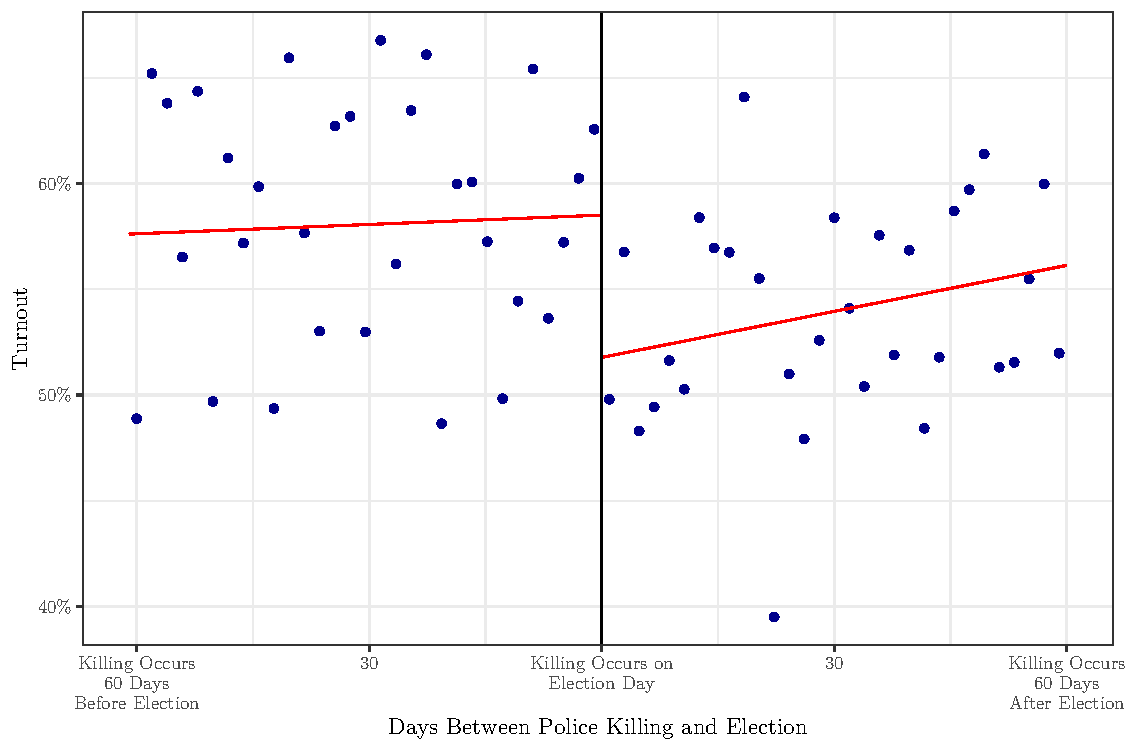
\includegraphics[width=\linewidth]{Figures/rd-plot-1} 
\caption{Regression Discontinuity Plot}
\subcaption*{Block Groups within 0.5 Miles of a Police Killing}
\label{fig:rdplot}

\end{figure}

Figure \ref{fig:rdplot} provides visual indication that police killings increase turnout when they occur in the weeks before an election. However, the figure does not indicate whether this observed discontinuity is statistically significant and it does not correct for demographic differences in block groups on either side of the cut-point. In Figure \ref{fig:diff-dist}, we plot the point estimates and 95\% confidence intervals for the 0.5-mile and other thresholds. As multiple block groups can be within the geographical threshold of a single killing---that is, multiple block groups can be ``treated'' by the same killing---robust standard errors are clustered by killing ID. At the far left of each panel, we test the discontinuity among block groups with 0.25 miles of a police killing before or after the election. We gradually expand that buffer by 0.05 miles at a time until reaching a 1-mile buffer. Weights are re-calculated each time new treated and control observations are included inside the buffer; these entropy balancing weights and OLS covariates are used in each model. In the left-most panel we plot traditional point estimates and confidence intervals; the middle panel presents the bias-corrected estimates; and the right-most panel uses the robust approach. In each case, we use the MSE-optimal bandwidth and a triangular kernel function.

\begin{figure}[!t]

{\centering 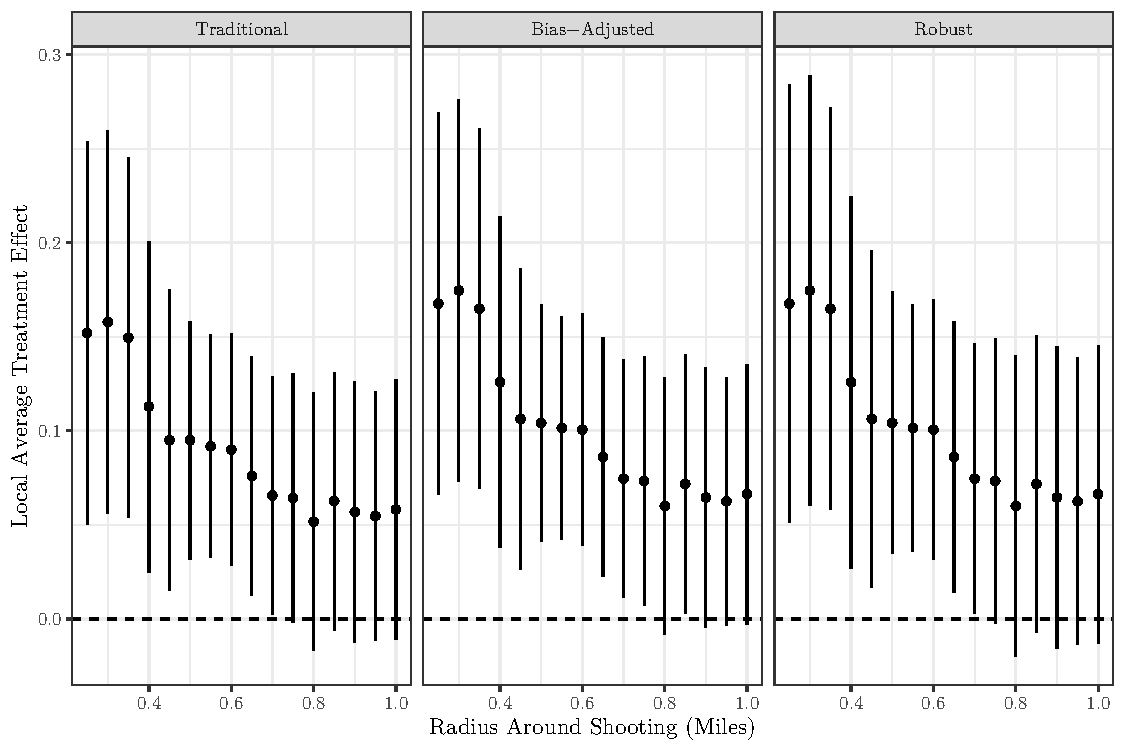
\includegraphics[width=0.9\linewidth]{Figures/dists-1} 

}

\caption{\label{fig:diff-dist}LATE By Distance from Killing}
\end{figure}

Figure \ref{fig:diff-dist} makes a number of things immediately clear. First, as expected, the local average treatment effect (LATE) of a police killing on turnout is highly geographically concentrated. The block groups closest to police killings saw their turnout increase \textit{dramatically}---by as much as 10 to 15 percentage points. This LATE---which is statistically significant at the 95\% level of confidence for block groups near killings---decays relatively quickly, however. By the time block groups whose centroids were a mile from the killing are included, the point estimate has dropped by roughly two-thirds and is no longer statistically significant. The figure also demonstrates that these estimates are robust to different estimation strategies. Figure \ref{fig:diff-dist} provides strong evidence in favor of Hypothesis H1c: police killings appear to substantially increase turnout, but these effects are highly geographically constrained.

\kscomment{I feel like you've done some number of robustness checks here. They need to be briefly summarized here.Do they show the same things aka are the results robust?}\kmcomment{I've tried to include notes to the SI above where I detail our modeling choices, saying that they don't really matter. After I say we use a polynomial of 1, for instance, I point to the SI; same with the entropy weights and OLS covariates. Hopefulyl I've made that clear enough in this pass that it'd be redundant to include them here.}


%\section*{Rallying Around the Flag or a Pursuit of Change?}
\section*{Group and Place Based Mobilization}
%\kscomment{Because I'm an asshole: One extension IF NEEDED AND THIS IS LIKELY OVERKILL of this could also be to compare pre and post BLM mobilization. \url{https://homicide.latimes.com/officer_involved/true}...I'm a little pissed that they didn't do this. Again, I realize this is overkill and just tell me that this is a stupid idea. This may also fall into the ``might be good for a different project or short paper'' category.}
%\kmcomment{do you mean whether the effects are bigger in 2020 (after 4 additional years of BLM) than they were in 2016? The treatment effects are actually smaller in 2020, but follow the same shape. Another thought, though, is whether police killings that occurred before / after Floyd was murdered had different effects (though this would have to be a registration test, since we aren't including May / June killings in our turnout tests)} \kscomment{No more like we'd need data on shootings pre 2013 and in the post 2013 world and compare. Again, I realize that this would be a gratuitous add to this paper at this point and be a lot more work.}\kmcomment{Gotcha. Unfortunately 2014 is the earliest snapshot of the registered voter file that I have so we can't get back any further!}

%\kscomment{Initial thoughts from e-mail chain: \\ 4. Possibly Theory Part 2: Discuss activism and registration. (Do we move this into point 2?) \\ 5. Registration Test (Do we put both tests in a single section?)} \kmcomment{I think the registration part belongs with the turnout stuff. Even though registrations increase, it doesn't really demonstrate which mechanism is at play. Don't have strong feelings on this though.}

    %\item \kscomment{From e-mail: Further, we might expect that those either already active in other areas from within the community or those active in this specific issue area from outside the community might turn to their traditional forms of organizing, such that they might now only push to get out the vote but also seek to register new voters. In other words, this suggests that other traditional tools and activities of those entrenched in political activism would also be brought to bare. One specific tool is registration. Thus, we also expect that voter registration numbers would increase  in communities where a police killing recently occurring (H2).}
    %\item \kmcomment{From e-mail: Okay, fine, there’s a mobilizing effect, but we don’t know what it is. I think this is where we set up dueling hypotheses about rally-round-the-flag vs contesting the state}
    %\item \kscomment{My vote would be that we just extend the implications from the place-based mobilization piece here + inject some interest group/social movements stuff. Essentially, we say that we find mobilizing affects indicating that the third piece is key to our understanding, which implies that we should see increased registration and that there are heterogeneous race affects. In other words, we can start to unpack the mechanisms by which this happens. Further, if we find heterogeneous race affects, then we can claim that really what we're showing is not in conflict with H1a but rather a complement to it, as we show that narrative likely matters but the type of contact also shapes the response.}

In the previous section we provide evidence that local communities are highly mobilized to vote by a police killing that occurs immediately before election. This overall, local average treatment effect, however, leaves many questions unanswered: Are these effects concentrated in Black communities, as past literature would suggest? Are these effects short-term responses by individuals, or do the police killings enter into longer-run politicization of communities? And finally, is increased turnout reflective of an electorate \textit{supportive} of a state they perceive to have kept them safe, or are voters registering \textit{discontent} with the government in the wake of an extrajudicial killing? In other words, although we now know \texit{that} extreme examples of police violence increase turnout, but we do not know \textit{why}.

As discussed above, recent scholarship on the power of narratives surrounding the criminal legal system \kmcomment{I realize that I've been going back and forth btwn CLS and carceral state. I'm fine using them interchangeably but that might be considered sloppy} can provide insight into how these events might be politicized. Specifically, work from Hannah Walker (2019; 2020) argues that contacts with the criminal legal system that are generally demobilizing can be mobilizing when understood in the context of particular narratives. She explains: ``experiences with punitive policies are subject to interpretation and, when understood through narratives of injustice, lead to wholly different participation outcomes than we usually predict,'' raising ``the possibility for political resistance'' \citep[][132-133]{walker2019targeted}. While Walker's work is specifically focused on the effects of proximal---not community---contact, the political threat literature would indicate that these narratives could equally extend beyond those in close personal relationship with those impacted by the carceral state. In a study demonstrating that some Arab-Americans are mobilized when faced with governmental discrimination, Tam Cho and colleagues sum up this literature: ``A solid body of evidence... indicates that political mobilization is a direct response to the degree of threat and discrimination a group experiences'' \citep[][978]{TamCho2006a}. It seems likely that in the years since the killing of Michael Brown and the growth of the Black Lives Matter movement, these narratives about the racist nature of police killings would have national salience. If these narratives about the carceral state extend to the local community---that is, if they feel that a local police killing is evidence of government discrimination against them, whether they knew the victim or not---there is strong reason to expect that the previously-identified turnout effects will be concentrated in Black neighborhoods and following the killing of a Black victim (\textit{H2}).

The existing literature on both criminal legal narratives and political threat also indicate that these effects are likely to be fairly durable; in other words, insofar as the narratives surrounding police killings are in fact salient and politically mobilizing, local organizers might incorporate them into longer-run political activity. Unfortunately, our RDiT cannot test the long-run turnout effects of a police killing. Instead, the causal framework can only estimate the turnout effects of block groups near a killing immediately before election day. To test the durability of a police killing on electoral political participation, we thus turn to a different activity: namely, voter registration. We use the registered voter file to calculate the number of registrations that occurred in each week in each block group, testing whether the weekly count increases following a police killing in the 6 months prior to the 2020 registration deadline. We expect to find an increase in registrations immediately following the police killing (\texit{H3}), reflecting a quick politicization of the killing. We also expect to find an increase in registrations shortly before the registration deadline regardless of when the killing occurred, which would reflect a community-wide incorporation of the killing into baseline political behavior, individually and / or through the actions of political activists organizing the sorts of registration drives common shortly before book-closing (\textit{H4}).

Finally, the political threat literature indicates that voters who feel targeted by ``worrisome government policy action'' \citep[][977]{TamCho2006a}---of which an extrajudicial killing is perhaps the most extreme example---view the ballot box as an apt venue for registering their anger \citep[e.g., ][]{White2016, Zepeda-Millan2017, Towler2018}. This surge in turnout, then, more likely reflects anger with---and not affirmation of---the state's practices. As such, we expect that geographical proximity to a police killing in Minneapolis will be associated with support for abolishing that city's police department in the 2021 ballot initiative (\textit{H5}).

%\begin{itemize}
%    \item We show that there is a mobilizing effect. However, that still leaves open the question of why. Both Walker's work and the theory of place-based mobilization give us an answer: narratives that indicate that it's a government source and that your community has been targeted. 
%    \begin{itemize}
%        \item Talk about narratives (see initial theory for the core of what this looks like). 
%        \item Sources: https://link.springer.com/article/10.1007/s11109-018-9461-9
%        \item \kmcomment{My paper on the neighborhood spillover effects of FD could be helpful, too. Imprisonment and disenfranchisement are obviously different than police violence but still the state exerting its influence: https://journals.sagepub.com/doi/10.1177/1078087420921522} \kscomment{\url{https://journals.sagepub.com/doi/full/10.1177/1078087420921522?casa_token=n8Ng3Sw6YrwAAAAA\%3A7L_Uu2WMtLyhtCIs1JoXEWeerOLQyC2g6mFlIC0LNzoASnPTdTJINUsw66pZ08zaAoJAcxsMbJPdDg}}
%    \end{itemize}
%    \item On the targeted bit, this implies that: (1) Black folks will mobilize at higher rates; and (2) People are more likely to mobilize if a Black individual is killed. 
%    \item On the ties to government, we would expect mobilization on policy specific ballot measures in addition to just a general turnout affect. This implies that: Folks will vote for anti-police measures at higher rates.
%    \item Options for reg: 
%    \begin{itemize}
%        \item We move it back up to the previous sections. If we do, then we likely gloss over the wonky things about reg and add it back to the previous test/initial section.
%        \item OR we add it here as a ``we'd expect it to affect other forms of participation as well, so let's look at registration." Then we *might* note some of its oddities but mostly sweep them under the rug. 
%        \item OR we argue that if communities tap into this broader framework and organize, it's unlikely to be a one-off short lived thing. Instead we'd expect long-run effects. While it's difficult to tell this with an event that's significantly time constrained, we may be able to test this with respect to a longer term activity with fewer time constraints: registering to vote. Here we'd expect LONG TERM EFFECTS ON REGISTRATION. This points to organizing happening within the community or the local community getting plugged into broader organization efforts. 
%        \item \kmcomment{We could also set up competing registration hypotheses here. Conditional on finding a registration effect, we expect to see it A) immediately following the killing, or B) later and closer to the registration deadline. As we've discussed we don't have *awesome* insight into how these mechanisms play out, but do have ideas about their interpretation (knee-jerk vs sustained). But I'm still not clear on how, say, an immediate effect would support one interpretation of the role of narratives and a later effect would point to something else. I get the durability piece, less clear on how it relates to the role of narratives and place-based mobilization. Seems like either an immediate or delayed effect could point to narratives and place-based mobilization}
%    \end{itemize} 
%    %\item What else?
%\end{itemize}

\subsection*{Differential Degrees of Mobilization by Race}

%\begin{itemize}
%    \item By race analysis
%    \item Key Take-Aways: (1) Statistically significant for predominately Black areas but not for less Black areas; (2) Substantively distinct relationships w/a larger substantive relationship being detected for predominately Black areas.
%\end{itemize}

Figure \ref{fig:by-race} asks whether the regression discontinuity estimates presented in the previous section differ based on the racial composition of the neighborhood (Panels (a) and (b)) or by the race of the victim (Panels (c) and (d)).\footnote{The victim's race was unknown for roughly 9\% of victims occurring within 2 months of the 2016 or 2020 elections. These observations are not included in the figure.} Figure \ref{fig:by-race}(a) indicates that the LATE differs markedly depending on the composition of the neighborhood, with substantially larger effects in plurality-Black block groups. The patterning of the coefficients in these block groups is striking in Panel (a): We see no evidence of immediate spatial decay in these block groups, and even plurality-Black block groups whose centroids are a mile from the nearest killing see turnout increase by as much as 15 percentage points. Latinx neighborhoods very close to a police killing see much higher turnout, though these effects abate quickly with distance. In no case are the estimates for plurality-white neighborhoods statistically significant, though they too trend toward zero as they become further removed from the nearest killing. In Panel (b), we show that the LATE for plurality-Black neighborhoods only approaches zero for block groups that are 7 or 8 miles from the nearest police killing.

Figure \ref{fig:by-race} also uncovers marked heterogeneity by the victim's race, particularly for Black victims. Mirroring Panels (a) and (b), we see that the spatial decay of a mobilizing LATE attributable to a police killing is far slower for Black than for non-Black victims. Panel (c) shows that Latinx victims are not mobilizing at a statistically significant level, but the relatively small number of these victims reduces the power of this analysis. The coefficients, however, exhibit the same spatial decay discussed previously. White victims follow a similar pattern. In Panel (d) we show once again that the LATE for Black victims does not drop to 0 until block groups are about 8 miles removed from the nearest killing. These findings provide strong evidence in support of H2. Though we cannot directly observe the influence of narratives on turnout following a police killing, the effects are strongly concentrated in precisely the places where we would expect narratives about racial injustice in the criminal legal system to be most mobilizing.

\begin{figure}[!t]
     \centering
     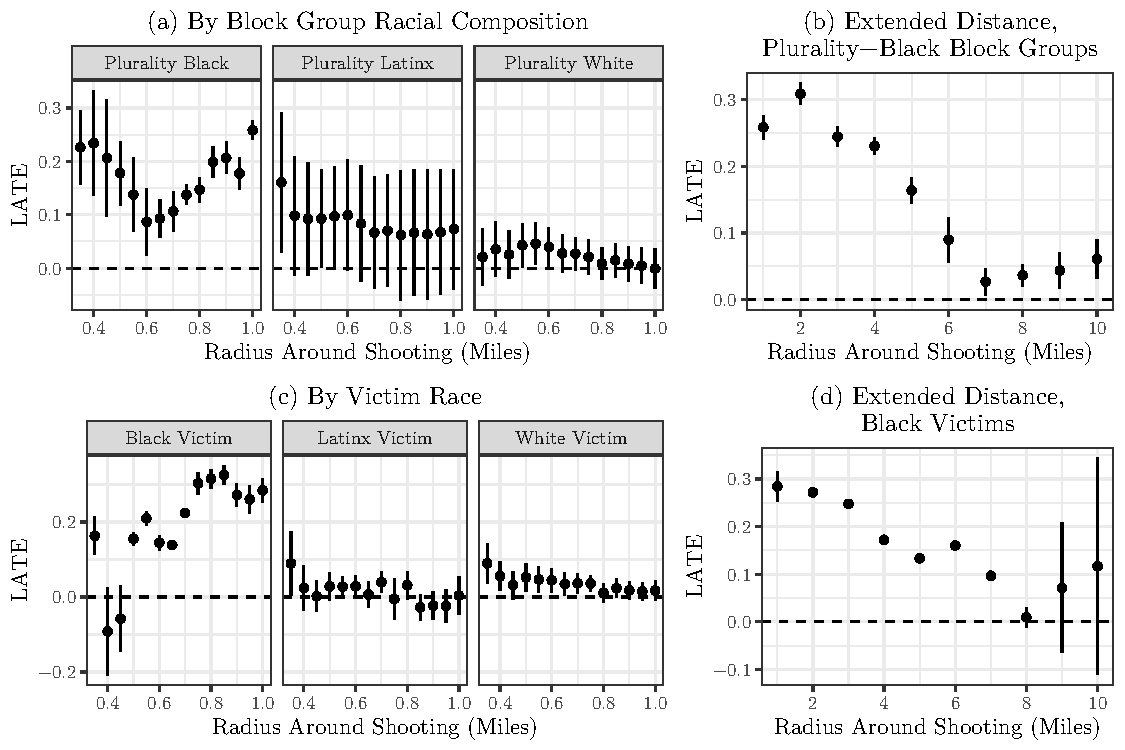
\includegraphics[width=\textwidth]{Figures/paneled-race-effects-1.pdf}
     \caption{LATE by Distance from Killing by Race}
     \label{fig:by-race}
     \subcaption*{\footnotesize \textit{Note:} Results in each subfigure come from regression discontinuity estimates similar to those presented in Figure \ref{fig:diff-dist} but run only on subsets of block groups. In each case, estimates include OLS covariates: \% white, \% Black, \% Asian, \% Latinx, median income, median age, population density, turnout in previous midterm election. In subfigures (a) and (b), we test whether there are heterogeneous affects based on the racial composition of block groups. In subfigures (c) and (d), we test whether there are heterogeneous affects based on race of the victim. While in the models producing subfigures (a) and (c) show the LATE for block groups whose centroids are up to 1 mile from a police killing, subfigures (b) and (d) include block groups up to 10 miles from the nearest police killing. \kscomment{This potentially gets moved partially into the text rather than here.}}
\end{figure}

\subsection*{Voter Registration}

Having established that police killings increase turnout in nearby block groups, and that these effects are especially concentrated in Black block groups and when the victim is Black, we now ask whether the democratic consequences of extrajudicial killings by the state extend to another form of electoral participation: namely, whether an individual decides to register to vote. Using voters' registration date from the voter file allows us to test whether the number of registered voters increases following a police killing. In addition to allowing us to test the effect of a police killing on a second form of participation, looking at weekly registration counts allows us to more finely explore the \textit{temporal} effects of police killings by examining whether any observed increase in registrations occurs immediately following the killing, or closer to the registration deadline when most voters actually register. The latter would point to a more durable politicizing effect of a police killing, whether attributable to individuals incorporating the killing into their baseline political socialization or to activists targeting these neighborhoods for registration drives even months after the killing.

We look specifically at the number of weekly registrations recorded in the registered voter file in each block group in each week for the 26 weeks ending with the voter registration deadline in each state in 2020. We thus have a balanced panel of all block groups, though the \textit{calendar} dates these weeks represent differ based on state-level registration deadlines. We estimate the treatment effect using a two-way fixed effects (TWFE) model, with fixed effects for block groups and weeks-before-registration-deadline. Block groups are considered treated following a police killing that occurred within 0.5 miles of its centroid. We use the \texttt{did} package in R, which allows for treatment effect heterogeneity and dynamics as detailed in \cite{Callaway2021}.\footnote{Because the calendar and relative-to-registration-deadline dates are not the same for each state (a killing in a state with election day registration, for instance, could occur \textit{earlier} relative to election day but on a \textit{later} calendar date than a killing in a state with an early registration deadline), only block groups that are never treated are allowed to serve as controls. For example, an officer killed an individual in Madison Heights, MI, on October 2. In Michigan, the registration deadline is election day, meaning this killing occurred in the 22nd week of the panel. In contrast, there was a police killing in Tempe, AZ, on September 25. Although this occurred earlier than the Michigan killing on the calendar, the earlier registration deadline in Arizona meant that it occurred in the 24th week of the data.\kmcomment{not really sure if the example is helpful or necessary}} In addition to the fixed effects, we include controls for block group characteristics including median income; share non-Hispanic white, non-Hispanic Black, Latinx, and Asian; median age; and population density. We cluster robust standard errors by both the block group ID, as well as the ID of the police killing by which they were treated.

Figure \ref{fig:twfe} presents two different ways of exploring the estimated treatment effect of police killings on voter registration. In Panel (a), we plot both the pre-treatment estimates and the estimated treatment effect by length of time since treatment. The pre-treatment estimates are what we would expect---the point estimates are small, non-significant, and there is no pattern to them. The post-treatment estimates indicate that there are positive treatment effects many weeks after a police killing occurs.

\begin{figure}[!t]
    \centering
    \subfloat[\centering Weeks Since Treatment]{{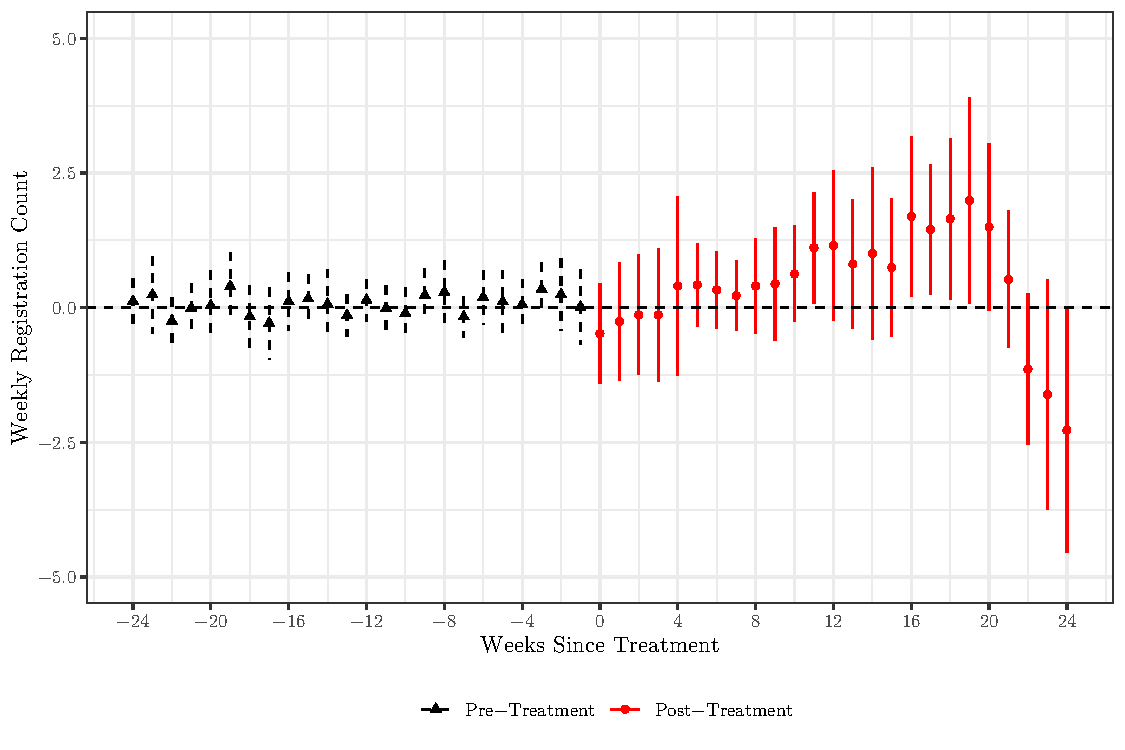
\includegraphics[width=.75\linewidth]{Figures/did-length-1.pdf} }}
    \qquad
    \subfloat[\centering Week of Year]{{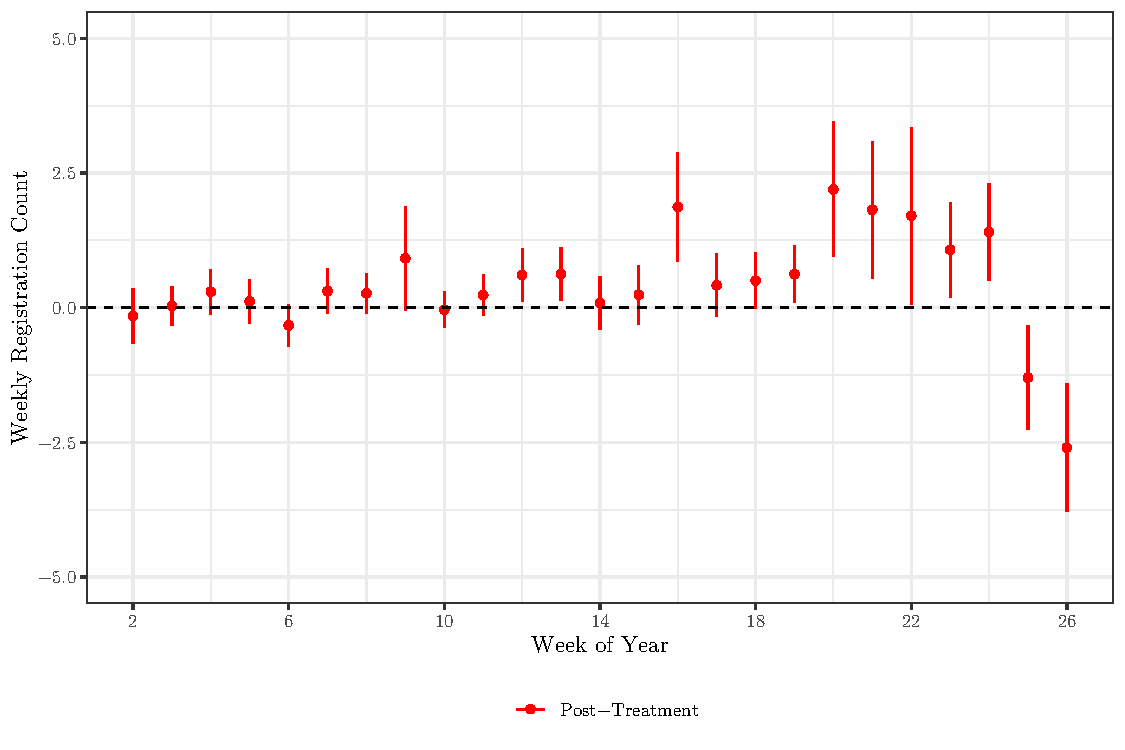
\includegraphics[width=.85\linewidth]{Figures/did-week-1.pdf} }}
    \caption{TWFE Estimates of Police Killings on Registration, 2020}
    \subcaption*{\kmcomment{I feel like the funkiness in the last two weeks could be driven by the SDR states so want to see what this looks like without them}}
    \label{fig:twfe}
\end{figure}

Of course, the estimated treatment effects for later periods in Panel (a) bump up against the registration deadlines for participation in the 2020 election. As such, we also plot the estimated treatment effect in each week of the year in Panel (b) of Figure \ref{fig:twfe}. Here, the story becomes much clearer: in the weeks before the registration deadline there is a significant increase in the weekly registration count (though this is not true of the very final 2 weeks). In the 7th through 3rd weeks before the registration deadline, the treatment effect averages an additional 1.64 registrations per week. Given that the average post-treatment block group actually had about 8.35 registrations in those weeks, this corresponds to roughly a 24\% increase in weekly registrations attributable to the police killing. While the \textit{average} treatment effect of a police killing on weekly registration counts is not statistically significant (that is, the killing does not raise registrations in enough post-treatment weeks to lead to an overall treatment effect), block groups subjected to extreme police clearly register more voters in the final weeks before book-closing.

Figure \ref{fig:twfe} makes clear that police killings seem to increase the weekly count of registrations in neighborhoods whose centers were close to a police killing in 2020. This effect, however, is concentrated near the registration deadline. This indicates that police killings enter into a community's baseline political socialization, pointing to a political effect that is relatively durable. To be sure, the precise causal mechanism by which registrations increase is not clear from this test; we cannot know whether individuals incorporated the police killing into their own political socialization, or if activists focused on block groups subject to extreme police violence when running registration drives in the weeks preceding the registration deadline. Regardless of \textit{how} this effect came about, it indicates that any politicizing effect of a police killing is not merely a momentary response, but can instead impact political behavior months later. Finally, although registration and turnout are substantially different activities, the apparent durability of the effect of police killings on registration might make the turnout effects estimated in the regression discontinuity models more generalizable beyond a local average treatment effect concentrated only in block groups near a police killing immediately before a presidential election. While we do not find support for H3 (registration does not immediately increase following a police killing), our evidence does support H4 with expected increases in registrations in the final weeks before the deadline.

%\kscomment{I think this points to \textit{either} a personal mobilizing affect or a more sustained or coordinated reform effort. We can't disentangle this. Essentially, it's not just a gut reaction. As this is the case, my gut says we actually revert the ordering. (1) competing t/o hypotheses; (2) t/o test; (3) implications -- resonance of message, support for policing reform, registration. To me, combined they tell a compelling story that it's not really an individual by individual thing but rather a community resonance structured by societal level narratives...which is still a bit of a reach based on what we show and differs from your interpretation.}\kmcomment{this seems right to me. I wasn't thinking about the possibility that activists could also be more mobilized to register people in areas with police killings months later. I'm fine with moving it later, agree that we say that we can't tell precisely *why* it's happening so much later but the fact that it *is* points to something interesting.}

\subsection*{Increased Support for Abolishing the Police}

As discussed above, it is not immediately clear how to contextualize these increases in turnout and registration. Are these citizens who feel protected by the state and have been reminded of its ability to keep them safe, whose political efficacy has increased along with the exhibition of state power? Or are these individuals who are made to feel \textit{unsafe} by an extrajudicial killing, the state taking the life of a resident without due process, turning to the ballot box to hold the state accountable?

To answer this question, we turn to a local election in Minneapolis, Minnesota, in the fall of 2021. In 2020, a Minneapolis Police Officer murdered resident George Floyd. Floyd's murder was captured on video and sparked the largest wave of protests in the history of the United States \citep{Buchanan2020}. Minneapolis had failed to implement recommended police reforms in the years prior to Floyd's murder \citep{Lartey2020}. In the aftermath of the protests, the Minneapolis City Council moved to abolish the Minneapolis Police Department and replace it with a different agency. This proposal came before Minneapolis voters as a ballot initiative in November, 2021, but failed to pass with 44\% of voters casting their ballots in favor of police abolition.

Although the ballot initiative did not pass, it can still offer insight into how citizens exposed to police violence respond politically to extrajudicial killings. We use precinct-level results from the ballot initiative to test whether precincts closer to a police killing opposed abolition at higher rates (supporting the Rally-Around-the-Flag hypothesis) or supported abolition at higher rates (providing evidence that police killings sour Americans on the handling of criminal justice issues).

In the regression below, the dependent variable is the share of voters in a precinct who supported abolishing the police department, and the key independent variable is the distance between the precinct's centroid and the nearest police killing between January 1, 2013 (the earliest date available in the Mapping Police Violence data) and the 2021 election. The police killed 11 individuals in Minneapolis during this time, 10 of which could be geocoded reliably.\footnote{The inclusion of the 11th, which was coded with 93.4\% accuracy, results in a higher point estimate that remains statistically significant at the 95\% level.} The demographics of each precinct are the average of the block groups in the precinct (either entirely or partially), weighted by the number of voters. Figure \ref{fig:minn-scatter} shows the bivariate relationship between distance to a police killing and support for abolition in 2021.

\begin{figure}[!ht]

\centering 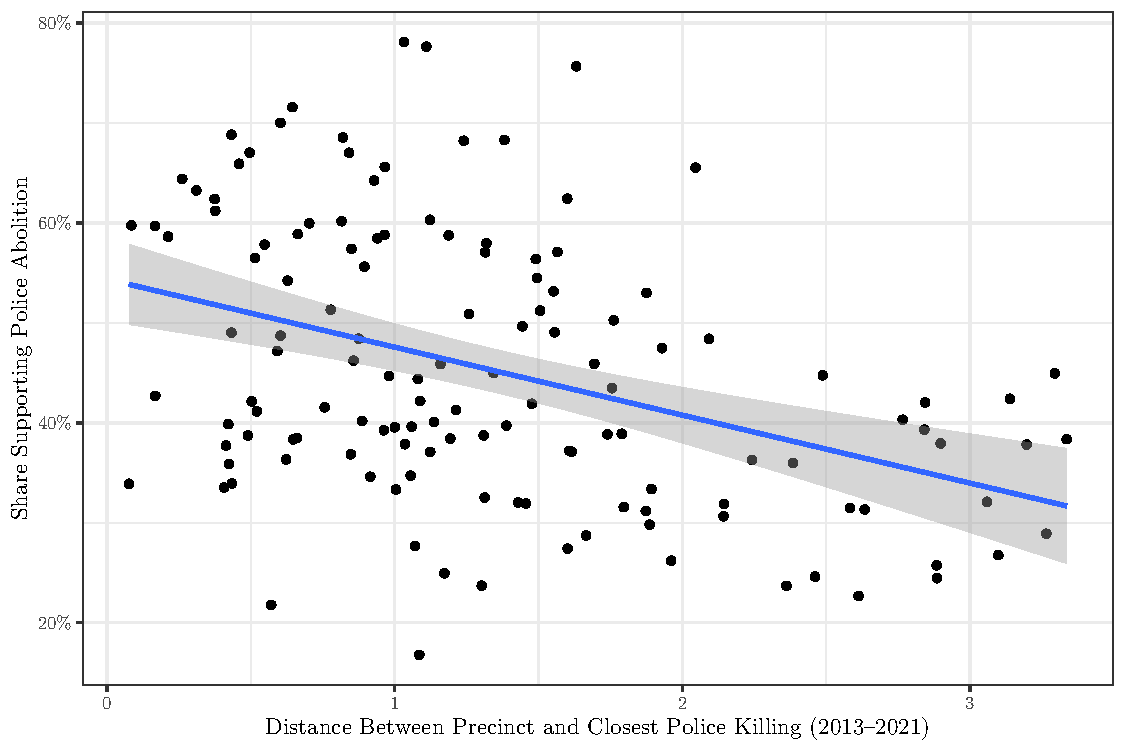
\includegraphics[width=\linewidth]{Figures/minn-scatter-1} 

\caption{\label{fig:minn-scatter}Support for Police Abolition and Distance to Police Killing}
\end{figure}

Police killings may be correlated with other exposure to the criminal legal system, which could be associated with support for police abolition. As such, we include the number of police stops in each precinct between January 1 and November 1, 2021. To control for underlying differences in the political preferences of different precincts, we also control for the voteshare won by Joe Biden in the 2020 presidential election one year earlier. As in earlier models, robust standard errors are clustered by the ID of the closest police killing to each precinct's centroid. These regressions are shown in Table \ref{tab:minn-reg-mini}.\footnote{For the full table, see the online appendix.} 

\begin{table}[t!]

\caption{\label{tab:minn-reg-mini} Support for Abolishing Minneapolis Police Department}

\centering
\begin{tabular}[t]{lccc}
\toprule
& Model 1 & Model 2 & Model 3\\
\midrule
Intercept & 0.544* & 0.453* & 0.322\\
& (0.032) & (0.116) & (0.189)\\
Distance to Closest Police Killing & -0.068* & -0.057* & -0.029*\\
& (0.022) & (0.018) & (0.011)\\
Logged Number of Police Stops in 2021 &  & 0.018 & -0.004\\
&  & (0.023) & (0.013)\\
Demographic Controls & N & N & Y \\
\midrule
Num.Obs. & 134 & 134 & 134\\
R$^2$ & 0.161 & 0.172 & 0.765\\
R$^2$ Adj. & 0.154 & 0.160 & 0.744\\
\bottomrule
\end{tabular}

\subcaption*{\footnotesize \textit{Note:} * indicates p $<$ 0.05. Standard errors clustered by nearest killing. Demographic controls include the percent of the population that is non-Hispanic Black, non-Hispanic white, Latinx, Asian, and with some college. Additionally, they include: median income, median age, logged population density, and Biden's 2020 vote share.}
\end{table}

As we can see, the relationship between distance to the closest police killing and support for abolition is large and statistically significant at the 95\% confidence level (Table \ref{tab:minn-reg-mini}). Net of other covariates, each additional mile between a precinct and a police killing is associated with a nearly 3 percentage point decrease in support for police abolition; put differently, precincts exposed to this sort of violence voted for the disbanding of the police at substantially higher rates. Somewhat surprisingly, the number of police stops in 2021 is entirely unrelated with a precinct's vote on the ballot initiative (\textit{p} = 0.43 in Model 2 and 0.77 in Model 3). While these cross-sectional regression estimates are not causal in nature, they are strongly consistent with the hypothesis that police killings lead citizens to use the ballot to hold the state accountable, and support H5.

\section*{Discussion}

Access to the ballot box has long been considered necessary for citizens seeking to protect themselves from an overzealous state. From the fight over the 15th Amendment following the Civil War, to the Civil Rights Era's focus on the Voting Rights Act of 1965, to contemporary organizing around the John R. Lewis Voting Rights Advancement Act, Black Americans have articulated the importance of voting to the securing of civil rights. In this manuscript, we provide novel evidence that these beliefs and narratives extend beyond national rhetoric and into the communities most impacted by extreme police violence. Ordinary Black Americans, it seems, also turn to the ballot box following the extrajudicial killing of a member of the community. Our exploration of registrations indicate that these effects are temporally durable, and the case study of Minneapolis implies that police violence undermines support for the police---and does so far more than quotidian police stops.

\begin{itemize}
    \item Recap
    \item (Academic) Contributions: 
    \begin{itemize}
        \item \textit{More generally on local mobilization:} Again drives home the role of narratives; Makes connections to prior movements and tactics that prior literature has not;
        \begin{itemize}
            \item From Before: \kmcomment{High level comment on the value of registration *and* turnout tests. Turnout is perhaps more substantively more important, BUT the registration test allows us to test like the temporal nature of the treatment. Is this an immediate / short lived thing, or is it more durable? Moreover, although the RDD can only estimate the LATE, I *think* that the registration test gives us a leg to at least gesture to the possibility that the LATE is more generalizeable, because we see registration effects even many many weeks after the treatment}
        \end{itemize}
        \item \textit{On criminal justice + political participation:} Directly tackles the diffuse space or tertiary-contact \kscomment{word choice} that has been little studied with respect to participation or observationally BUT that many have begun looking at using survey experiments. 
        \item Methods
    \end{itemize}   
    \item Limitations/Next Steps:
    \begin{itemize}
        \item Is violence distinct from other form of police interactions? Tie to experimental work. 
        \item Has this changed over time (i.e., in light of BLM)?
        
    \end{itemize}
    \item Broaden out the implications.
\end{itemize}

% References
\clearpage
\bibliographystyle{apsr}
\bibliography{Policing.bib, shootings_to.bib} % You can just add a second bib here by adding a comma and then name of your bib file.

\end{document}
